\documentclass[problem]{mcs}

\begin{pcomments}
  \pcomment{FP_seating_around_a_round_table}
  \pcomment{by Megumi F09}
  \pcomment{edited slightly by ARM S10}
\end{pcomments}

\pkeywords{
  combinatorics
  permutation
  division rule
  inclusion-exclusion
}

%%%%%%%%%%%%%%%%%%%%%%%%%%%%%%%%%%%%%%%%%%%%%%%%%%%%%%%%%%%%%%%%%%%%%
% Problem starts here
%%%%%%%%%%%%%%%%%%%%%%%%%%%%%%%%%%%%%%%%%%%%%%%%%%%%%%%%%%%%%%%%%%%%%

\begin{problem}
  The queen and king of hearts decide to host a poker game and
  invite their six fellow royals ---the queen and king of clubs,
  diamonds, and spades.  The queen of hearts has a round table with
  eight chairs $P_1, P_2, \dots, P_8$ for these eight people:
\begin{center}
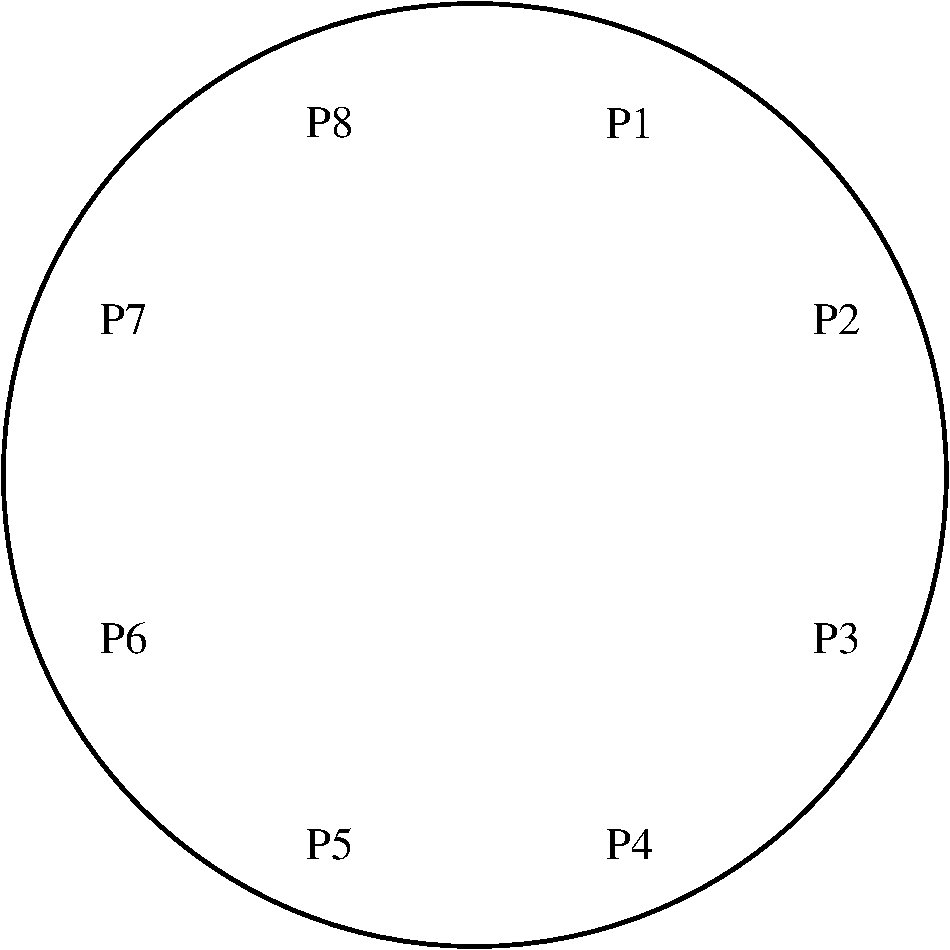
\includegraphics[height=2.0in]{figures/round_table.pdf}
\end{center}


%  for the guests (the $3$ other couples) and the host and hostess (her
%  husband and herself).

You may answer each of the following questions with a numerical
expression that uses factorials and arithmetic operations.

\bparts 
\ppart In how many ways can the queen assign the eight people to
different chairs?
\begin{center}
\exambox{0.7in}{0.4in}{0.2in}
\end{center}

%\hfill\examrule
%\examspace[0.5in]
\begin{solution}
$8!$
\end{solution}

\eparts
\examspace[0.3in]

A \emph{seating} is a circular arrangement of people around the table
in which all that matters is who sits next to whom, not which chairs
they are in.  In other words, two ways of assigning people to chairs
define the \emph{same seating} when one assignment is a rotation of
the other.  For example, the following two assignments of people to
chairs define the same seating:

\newcommand{\spa}{\spadesuit}
\newcommand{\hea}{\heartsuit}
\newcommand{\dia}{\diamondsuit}
\newcommand{\clu}{\clubsuit}

\[\begin{array}{|l|l|l|l|l|l|l|l|}
\hline
P_1 & P_2 &P_3 &P_4 & P_5 & P_6 & P_7 & P_8 \\ \hline \hline
K\spa & Q\spa & K\hea & Q\hea & K\dia & Q\dia & K\clu & Q\clu \\ \hline
K\dia & Q\dia & K\clu & Q\clu & K\spa & Q\spa  & K\hea & Q\hea \\ \hline 
\end{array}\]

%\begin{eqnarray*}
%K\spa, Q\spa, K\hea, Q\hea, K\dia, Q\dia, K\clu, Q\clu \\
%Q\hea, K\dia, Q\dia, K\clu, Q\clu, K\spa, Q\spa, K\hea 
%\end{eqnarray*}
%\end{definition}

\bparts

\ppart How many different \emph{seatings} are there?

\begin{center}
\exambox{0.7in}{0.4in}{0.2in}
\end{center}

% \hfill\examrule

\examspace[0.7in]
\begin{solution}
\[
\frac{8!}{8} = 7!
\]
\end{solution}

\inhandout{\instatements{\newpage}}

\ppart How many distinct \emph{seatings} are there if the queen and king of
hearts must be seated next to each other?
\hint Think of the queen and king as one unit, but remember the king and queen can be in either order.

%\hfill \examrule[0.75in]

\begin{center}
\exambox{0.75in}{0.5in}{0.2in}
\end{center}

\examspace[0.6in]
\begin{solution}
\[
2! \cdot \frac{7!}{7} = 2 \cdot 6!
\]
\end{solution}

\ppart How many distinct \emph{seatings} are there if the queen and
king of hearts must be seated next to each other, and the queen and
king of spades must also be seated next to each other?

\begin{center}
\exambox{1.5in}{0.5in}{0.2in}
\end{center}


%\hfill \examrule[0.75in]

\examspace[1.0in]
\begin{solution}
\[
2! \cdot 2! \cdot \frac{6!}{6} = 4 \cdot 5!
\]
\end{solution}

\ppart How many distinct \emph{seatings} are there where no one is
seated next to their spouse? 
%\hint Use inclusion-exclusion.

\hint Let $N_1$ be the answer to part~(c), $N_2$ the answer to part~(d), $N_3$ be the number of seatings with each of the $\spa$, $\hea$, and $\dia$ couples seated next to their spouses, and $N_4$ be the number of seatings with everyone next to their spouse.  Use inclusion-exclusion and express your answer in terms of the $N_i$'s. 

%\hfill\examrule[3in]

\begin{center}
\exambox{4.5in}{1.0in}{0.3in}
\end{center}

%\examspace[3in]
\begin{solution}
\begin{eqnarray*}
\mbox{Answer} &=& \{\mbox{Total seatings}\} \\
&-& \binom{4}{1} \times \{\mbox{Seatings with at least one couple seated together}\} \\
&+& \binom{4}{2} \times \{\mbox{Seatings with at least two couples seated together}\} \\
&-& \binom{4}{3} \times \{\mbox{Seatings with at least three couples seated together}\} \\
&+& \binom{4}{4} \times\{\mbox{Seatings with the four couples seated together}\} \\
&=& 7! - 4 \cdot (2 \cdot 6!) + 6 \cdot (4\cdot 5!) - 4 \cdot (8 \cdot 4!) + 1 \cdot (16 \cdot 3!)
\end{eqnarray*}
\end{solution}

\eparts
\end{problem}

%%%%%%%%%%%%%%%%%%%%%%%%%%%%%%%%%%%%%%%%%%%%%%%%%%%%%%%%%%%%%%%%%%%%%
% Problem ends here
%%%%%%%%%%%%%%%%%%%%%%%%%%%%%%%%%%%%%%%%%%%%%%%%%%%%%%%%%%%%%%%%%%%%%

\endinput
